%%%%%%%%%%%%%%%%%%%%%%%%%%%%%%%%%%%%%%%%%%%%%%%%%%%%%%%%%%%%%%%%%%%
% 
% $Id: sec4.tex,v 1.1.1.1 2002/01/02 19:36:48 phil Exp $
%
% $Log: sec4.tex,v $
% Revision 1.1.1.1  2002/01/02 19:36:48  phil
% initial import into CVS
%
% Revision 1.3  1997/09/06 19:17:48  allen
% *** empty log message ***
%
% Revision 1.2  1997/08/28 16:40:06  cguo
% *** empty log message ***
%
% Revision 1.1  1995/09/12 16:51:30  stockie
% Initial revision
%
%
%%%%%%%%%%%%%%%%%%%%%%%%%%%%%%%%%%%%%%%%%%%%%%%%%%%%%%%%%%%%%%%%%%%

\section{Accuracy of Difference Approximations}
\label{lab2:sec:first-deriv}  % this one kept around for posterity :^)
\label{lab2:sec:accuracy-main}

Before moving on to the details of how to measure the error in a
scheme, let's take a closer look at another example which we've seen
already \dots 

\begin{example}
  \label{lab2:exm:accuracy}
  Let's go back to the heat conduction equation from Lab~\#1,
  \externalref{lab1:exm:conduction} where the temperature,
  $T(t)$, of a rock immersed in water or air, evolves in time
  according to the first order ODE: 
  \begin{equation}
    \frac{dT}{dt} = \lambda(T,t) \, (T-T_a) 
    \label{lab2:eq:conduction}
  \end{equation}
  with initial condition $T(0)$. 
  We saw in the section on the forward Euler
  method~\externalref{lab1:sec:forward-euler} that one way to
  discretize this equation was using the forward difference
  formula~\eqref{lab2:eq:forward-diff}  
  for the derivative, leading to
  \[
  T_{i+1} = T_i + \Delta t \, \lambda(T_i,t_i) \, (T_i-T_a).
  \]
  Similarly, we could apply either of the other two difference
  formulae, \eqref{lab2:eq:backward-diff} or
  \eqref{lab2:eq:centered-diff}, to obtain other difference schemes,
  namely what we called the \emph{ backward Euler method}
  \[
  T_{i+1} = T_i + \Delta t \, \lambda(T_{i+1},t_{i+1}) \, (T_{i+1}-T_a), 
  \]
  and the \emph{ leap frog method}
  \[
  T_{i+1} = T_{i-1} + 2 \Delta t \, \lambda(T_{i},t_{i}) \, (T_{i}-T_a). 
  \]
  The forward Euler and leap frog schemes are called \emph{ explicit
    methods}, since they allow the temperature at any new time to be
  computed in terms of the solution values at previous time steps.
  The backward Euler scheme, on the other hand, is called an \emph{
    implicit scheme}, since it gives an equation defining $T_{i+1}$
  implicitly (If $\lambda$ depends non-linearly on $T$, then this
  equation may require an additional step, involving the iterative
  solution of a non-linear equation.  We will pass over this case for
  now, and refer you to a reference such as 
  ~\cite{burden-faires} for the details on non-linear solvers
  such as \emph{ Newton's method}).

  For now, let's assume that $\lambda$ is a constant, independent of
  $T$ and $t$.
  Plots of the numerical results from each of these
  schemes, along with the exact solution, are given in
  Figure~\ref{lab2:fig:compare} (with the ``unphysical'' parameter
  value $\lambda=0.8$ chosen to enhance the show the growth of
  numerical errors, even though in a real material this would
  violate conservation of energy).
  \begin{figure}[htbp]
    \begin{center}
      \leavevmode
%%%%%%%%%%%%%%%%%%%%%%%%%%%%%%%%%%%%%%%%%%%%%%%%%%%%%%%%%
%  NOTE: This plot was produced using:
%            compare <in1 >out1  
%            compare <in1.exact >out1.exact
%            gnuplot <gin1
%  The source code for the program ``compare'' is 
%  ``compare.c'' (compiled with ``make compare'').
%%%%%%%%%%%%%%%%%%%%%%%%%%%%%%%%%%%%%%%%%%%%%%%%%%%%%%%%%
      \includegraphics[height=3.5in]{accuracy/compare1}      
      \caption{A plot of the exact and computed solutions for the
        temperature of a rock, with parameters: $T_a=20$, $T(0)=30$, 
        $\lambda= +0.8$, $\Delta t=\frac{1}{3}$.}
      \label{lab2:fig:compare}
    \end{center}
  \end{figure}
  
  Notice from these results that the centered scheme is the most
  accurate, and backward Euler the least accurate.  
\end{example}

The next section explains why some schemes are more accurate than
others, and introduces a means to quantify the accuracy of a
numerical approximation.

\begin{latexonly}
\gloss{forward Euler method}{a numerical method that uses forward
discretization for the time derivative(s).}
\gloss{backward Euler method}{a numerical method that uses backward
discretization for the time derivative(s).}
\gloss{explicit scheme}{the solution at a given time step depends only
on the solution value at previous time steps.}
\gloss{implicit scheme}{the solution at a given time step depends on
solution values of the current time step as well as previous time steps.}
\end{latexonly}
%%%%%%%%%%%%%%%%%%%%%%%%%%%%%%%%%%%%%%%%%%%%%%%%%%%%%%%%%%%%%%%%%%%%%%%
\subsection{Round-off Error and Discretization Error}
\label{lab2:sec:accuracy}

From Example~\ref{lab2:exm:accuracy} and the example in the Forward
Euler section of the previous lab,~\externalref{lab1:exm:saturation}
it is obvious that a numerical 
approximation is exactly that - \textbf{ an approximation}.
The process of discretizing a differential equation inevitably leads
to errors.
In this section, we will tackle two fundamental questions related to
the accuracy of a numerical approximation:
\begin{itemize}
\item Where does the error come from (and how can we measure it)?
\item How can the error be controlled?
\end{itemize}

\subsubsection{Where does the error come from?}

\paragraph{Round-off error:}

When attempting to solve differential
equations on a computer, there 
are two main sources of error.  The first, \emph{ round-off error},
derives from the fact that a computer can only
represent real numbers by \emph{ floating point} 
approximations, which
have only a finite number of digits of accuracy.
%%%%%%%%%%%%%%%%%%%%%%%%
\begin{latexonly}
\gloss{round-off error}{the error made by representing a real number
  as a floating-point number on a computer.  The floating point
  representation only has a finite number of digits, and the round-off
  error is the difference between the infinite-precision real number
  and its floating point approximation.}
\gloss{floating point}{the storage method that a computer uses to
  represent real numbers.  A decimal floating-point number has the
  form $\pm 0.d_1 d_2 d_3 \ldots d_k \times 10^n$,
  where each digit, $d_i$ is between 0 and 9 (except $d_1$, which must
  be non-zero).  Computers actually use a \emph{ binary} (or base 2)
  floating point representation.}
\end{latexonly}
%%%%%%%%%%%%%%%%%%%%%%%%

\begin{mathnote}
      \hyperref{Floating point representation of numbers.}{See Appendix }{ for a
      description of floating point representation of
      numbers.}{lab2:ap:floating-point} 
\end{mathnote}

\begin{example}
  For example, we all know that the number $\pi$ is a non-repeating
  decimal, which to the first twenty significant digits is
  $3.1415926535897932385\dots$
  Imagine a computer which stores only eight significant digits, so that
  the value of $\pi$ is rounded to $3.1415927$.
  
  In many situations, these five digits of accuracy may be sufficient.
  However, in some cases, the results can be catastrophic, as shown in
  the following example:
  \[
    \frac{\pi}{(\pi + 0.00000001)-\pi}. 
  \]
  Since the computer can only ``see'' 8 significant digits, the addition
  $\pi+0.00000001$ is simply equal to $\pi$ as far as the computer is
  concerned. 
  Hence, the computed result is $\frac{1}{0}$ - an undefined expression!
  The exact answer $100000000\pi$, however, is a very well-defined
  non-zero value.   
\end{example}

\paragraph{Truncation error:}

The second source of error stems from the discretization of the
problem, and hence is called \emph{ discretization error}
or \emph{ truncation error}. 
In comparison, round-off error is always present, and is independent
of the discretization being used.
The simplest and most common way to analyse the truncation error in a
scheme is using \emph{ Taylor series expansions}.  
\begin{mathnote}
  \hyperref{Some details on Taylor series\dots }{See Appendix }{ for a
    review of Taylor series.}{lab2:ap:taylor-series}
\end{mathnote}

Let us begin with the forward difference formula for the first
derivative, \eqref{lab2:eq:forward-diff}, which involves the discrete
solution at times $t_{i+1}$ and $t_{i}$.  
Since only continuous functions can be written as Taylor series, we
expand the exact solution (instead of the discrete values $T_i$) at the
discrete point $t_{i+1}$:
\[
  T(t_{i+1}) = T(t_i+\dt) = T(t_i) + (\Delta t) T^\prime(t_i) + 
  \frac{1}{2}(\Delta t)^2 T^{\prime\prime}(t_i) +\cdots,
%%+   \frac{1}{6}(\dt)^3   y^{\prime\prime\prime}(t_i) + \cdots
\]
We can then subtract $T(t_i)$ and divide the result by $\Delta t$ in
order to obtain
\begin{eqnarray}
  \frac{T(t_{i+1})-T(t_i)}{\Delta t} &=& T^{\prime}(t_i) +
  \underbrace{\frac{1}{2}(\Delta t) T^{\prime\prime}(t_i) + \cdots}
_{\mbox{\rm truncation error}} \nonumber \\ \; \nonumber \\
%%+    \frac{1}{6}(\dt)^2   y^{\prime\prime\prime}(t_i) + \cdots} 
  &=& T^{\prime}(t_i) + {\cal O}(\Delta t).
  \label{lab2:eq:disc-error}
\end{eqnarray}

\begin{note}
This second expression writes the truncation error term in terms of
\emph{ order notation}.  If we write $y = {\cal O}(\Delta t)$, then we
mean simply that $y<c \cdot \Delta t$ for some constant $c$, and we say
that ``\emph{ $y$ is first order in $\Delta t$}'' (since it depends on
$\Delta t$ to the first power) or ``\emph{ $y$ is big-oh of 
  $\Delta t$}.'' As  $\Delta t$ is assumed small, the next term in the 
series, $\Delta t^2$ is small compared to the $\Delta t$ term.
\end{note}

It is clear from \eqref{lab2:eq:disc-error} that as $\Delta t$ is
reduced in size (\ie as the 
computational grid is refined), the error is also reduced.  
If you
remember that we derived the approximation from the limit definition
of derivative,\externalref{lab2:eq:defn-deriv} then this should make
sense. 
This dependence of the error on powers of the grid spacing $\Delta t$
is an underlying characteristic of difference approximations, and we
will see approximations with higher orders in the coming sections
\dots 

%%%%%%%%%%%%%%%%%%%
\begin{latexonly}
\gloss{local truncation error}{or \emph{ truncation error}.  This is the
  error made in approximating the solution to an ODE over a single
  step.  A simple method for computing the actual form of the error is
  by Taylor series expansion.}
\gloss{global truncation error}{this is the
  error made in approximating the solution to an ODE over the entire
  course of the numerical integration.  It is typically more difficult
  to derive an analytical expression for this error than it is with
  the \emph{ local truncation error}.}
\gloss{truncation error}{the error made in approximating a continuous
  function by a discrete formula.  When talking about numerical
  approximations to ODE's, there are actually two types of
  truncation error: \emph{ global truncation error} and \emph{ local
    truncation error}.  When the term \emph{ truncation error} is used
  by itself, it usually refers to local truncation error.}
\gloss{discretization error}{see truncation error}
\end{latexonly}
%%%%%%%%%%%%%%%%%%%

There is one more important distinction to be made here.  The
``truncation error'' we have been discussing so far is actually what
is called \emph{ local truncation error}.  It is ``local'' in the sense
that we have expanded the Taylor series \emph{ locally} about the
exact solution at the point $t_i$.  

There is also a \emph{ global truncation error} (or, simply, \emph{
  global error}), which is the error made during the course of the
entire computation, from time $t_0$ to time $t_n$.  The difference
between local and global truncation error is illustrated in
Figure~\ref{lab2:fig:truncation-error}.
\begin{figure}[htbp]
  \begin{center}
    \leavevmode
%%%%%%%%%%%%%%%%%%%%%%%%%%%%%%%%%%%%%%%%%%%%%%%%
%  NOTE:  This figure was drawn in xfig 
%  (the figure file is ``images/error.fig'')
%  and then exported to an encapsulated 
%  postscript file.
%%%%%%%%%%%%%%%%%%%%%%%%%%%%%%%%%%%%%%%%%%%%%%%%
    \htmlimage{scale=1.5}
    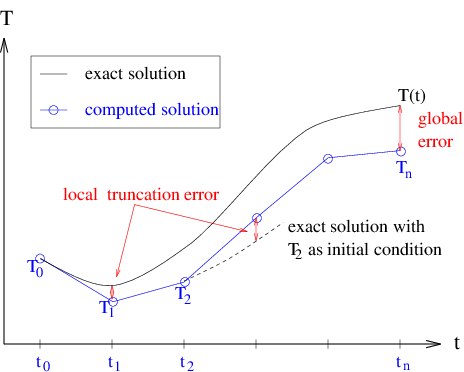
\includegraphics[height=3.0in]{images/error}
    \caption{Local and global truncation error.  }
    \label{lab2:fig:truncation-error}
  \end{center}
\end{figure}

It is easy to get a handle on the order of the local truncation
error using  Taylor series, regardless of whether the exact solution is
known, but no similar analysis is available for the global
error.  We can write
\[
\mbox{\rm global error} = |T(t_n)-T_n|
\]
(see Figure~\ref{lab2:fig:truncation-error}),  but this expression
can only be evaluated if the exact solution is known ahead of 
time (which is not the case in most problems we want to compute,
since otherwise we wouldn't be computing it in the first place!).
Therefore, when we refer to truncation error, we will 
always be referring to the local truncation error.

\begin{problem}
  \label{lab2:prob:taylor}
  \begin {itemize}
  \item a)
  Derive the error term for the backward difference formula
  \eqref{lab2:eq:backward-diff} using 
  Taylor series, and hence show that it is also first order.
  
   \item b)
  How does the constant in front of the leading order error term
  differ from that for the forward difference formula?  
  Relate this back to the results plotted in
  Figure~\ref{lab2:fig:compare}, where these two formulae were used to
  derive difference schemes for the heat conduction problem. 

  \item c)
  Repeat a) for the centered difference formula
  \eqref{lab2:eq:centered-diff}.  What is the order of this
  approximation to the first derivative?

  \end {itemize}
\end{problem}

\subsubsection{How can we control the error?}

Now that we've determined the source of the error in numerical
methods, we would like to find a way to control it; that is, we would
like to be able to compute and be confident that our approximate solution is
``close'' to the exact solution.
Round-off error is intrinsic to all numerical computations, and cannot
be controlled (except to develop methods that do not magnify the error
unduly \dots\ more on this later).  
Truncation error, on the other
hand, \emph{ is} under our control.
\begin{note}
  In the simple ODE examples that we're dealing with in this lab, the
  round-off error in a calculation is much smaller than 
  the truncation error.  Furthermore, the schemes being used are \emph{
    stable with respect to round-off error} in the sense that
  round-off errors are not magnified in the course of a computation.
  So, we will restrict our discussion of error control in what follows
  to the truncation error.

  However, there are many numerical algorithms in which the  round-off
  error can dominate the the result of a computation (Gaussian
  elimination is one example, which you will see in
  Lab~\#3~\externalref{lab3:sec:round-off-error}), and so we must
  always keep it in mind when doing numerical computations. 
\end{note}

There are two fundamental ways in which the truncation error in an
approximation~\eqref{lab2:eq:disc-error} can be reduced: 
\begin{enumerate}
\item Decrease the grid spacing, \dt.  
  Provided that the second derivative of the solution is bounded, it
  is clear from the error term in~\eqref{lab2:eq:disc-error} that as \dt\ 
  is reduced, the error will also get smaller.  This principle was
  demonstrated in an example from
  Lab~\#1.\externalref{lab1:exm:saturation} 
  The disadvantage to decreasing \dt\ is that the cost of the
  computation increases since more steps must be taken.
  Also, there is a limit to how small \dt\ can be, 
  beyond which round-off errors will start
  polluting the computation.
\item Increase the order of the approximation.
  We saw above that the forward difference
  approximation of the first derivative is first order accurate in the
  grid spacing.  It is also possible to derive higher order difference
  formulas which have a leading error term of the form $(\dt)^p$,
  with $p>1$. 
  You should have discovered already in Problem~\ref{lab2:prob:taylor}
  that the centered difference formula
  \eqref{lab2:eq:centered-diff} is a second order scheme, and some
  further examples will be given in 
  Section~\ref{lab2:sec:highorder-taylor}.
  The main disadvantage to using very high order schemes is that the
  error term depends on higher derivatives of the solution, which can
  sometimes be very large -- in this case, the stability of the scheme
  can be adversely affected (for more on this, see
  Section~\ref{lab2:sec:stability}). 
\end{enumerate}

\begin{problem}
  \label{lab2:prob:accuracy}
  In order to investigate these two approaches to improving the
  accuracy of an approximation, you can use the code in terror2.m
  or terror2.py to play with the solutions to the heat conduction equation.
  For a given function $\lambda(T)$, and specified parameter values,
  you should experiment with various time steps and schemes, and
  compare the computed results (Note: only the answers to the assigned
  questions need to be handed in).   Look at the different schemes
  (euler, leapfrog, 4th order runge kutta) run them for various
  total times (tend) and step sizes (dt=tend/npts).

  The three schemes that will be used here are forward Euler (first
  order), leap frog (second order) and the fourth order Runge-Kutta
  scheme (which will be introduced in
  \htmladdnormallink{Lab~\#4}{\LabfourURL}).  

  To hand in:  Try three different step sizes for all three
  schemes for a total of 9 runs.  It's helpful to be able to change
  the axis limits to look at various parts of the plot. In matlab
  you do that with a sequence like

\begin{verbatim}
figure(1);  %make figure 1 current
ax=gca;     %get the current  axis
set(ax,'ylim',[-10,50]);  %set the y limits
set(ax,'xlim',[0,1]);  % zoom in on the first second
\end{verbatim}

Use your 9 results to answer parts a and b below.  (The leap-frog
scheme should give you quasi-pathological results, see the explanation at
the end of section 5)


  \begin {itemize}
  \item a) Does increasing the order of the
    scheme, or decreasing the time step always improve the solution?
  \item b) How would you compute the local truncation error from the
    error plot?  And the global error?  Do this on a plot for
    one set of parameters.
  \item c) Similarly, how might you estimate the \emph{ order} of the local
    truncation error?  The order of the global error? (\textbf{ Hint:} An
    order $p$ scheme has truncation error that looks like
    $c\cdot(\Delta t)^p$.  Read the error off the plots for several
    values of the grid spacing and use this to find $p$.)  
    Are the
    local and global error significantly
    different?  Why or why not?
  \end{itemize}
\end{problem}

%%%%%%%%%%%%%%%%%%%%%%%%%%%%%%%%%%%%%%%%%%%%%%%%%%%%%%%%%%%%%%%%%%%%%%%
\subsection{Other Approximations to the First Derivative}
\label{lab2:sec:other}

The Taylor series method of deriving difference formulae for the first
derivative is the simplest, and can be used to obtain approximations
with even higher order than two.  There are also many other ways to
discretize the derivatives appearing in ODE's, as shown in the
following sections\dots

%%%%%%%%%%%%%%%%%%%%%%%%%%%%%%%%%%%%%%%%%%%%%%%%%%%%%%%%%%%%%%%%%%%%%%%
\subsubsection{Higher Order Taylor Methods}
\label{lab2:sec:highorder-taylor}

As mentioned earlier, there are many other possible approximations to
the first derivative using the Taylor series approach.  The basic
approach in these methods is as follows:
\begin{enumerate}
\item expand the solution in a Taylor series at one or more points
  surrounding the point where the derivative is to be approximated
  (for example, for the centered scheme, you used two points,
  $T(t_i+\dt)$ and $T(t_i-\dt)$.  You also have to make sure that you
  expand the series to a high enough order \dots 
\item take combinations of the equations until the $T_i$ (and possibly
  some other derivative) terms are
  eliminated, and all you're left with is the first derivative term.
\end{enumerate}
One example is the fourth-order centered difference formula for the first
derivative:
\[
  \frac{-T(t_{i+2})+8T(t_{i+1})-8T(t_{i-1})+T(t_{i-2})}{12\dt} =
  T^\prime(t_i) + {\cal O}((\dt)^4)
\]

\textbf{Quiz:}  Try the quiz at 
\href{http://clouds.eos.ubc.ca/~phil/numeric/docs/_build/html/quizzes2/order.html}{this link} related to this higher order scheme.

%%%%%%%%%%%%%%%%%%%%%%%%%%%%%%%%%%%%%%%%%%%%%%%%%%%%%%%%%%%%%%%%%%%%%%%
\subsubsection{Predictor-Corrector Methods}
\label{lab2:sec:pred-corr}

Another class of discretizations are called \emph{ predictor-corrector
  methods}.  
Implicit methods can be difficult or expensive to use because of the
solution step, and so they are seldom used to integrate ODE's.
Rather, they are often used as the basis for predictor-corrector
algorithms, in which a ``prediction'' for $T_{i+1}$ based only on an
explicit method is then ``corrected'' to give a better value by using
this precision in an implicit method.  

To see the basic idea behind these methods, let's go back (once
again) to the backward Euler method for the heat conduction problem
which reads:
\[ 
T_{i+1} = T_{i} + \Delta t \, \lambda( T_{i+1}, t_{i+1} ) \, ( T_{i+1}
- T_a ).
\]
Note that after applying the backward difference formula
\eqref{lab2:eq:backward-diff}, all terms in the right hand side are
evaluated at time $t_{i+1}$.  

Now, $T_{i+1}$ is defined implicitly in terms of itself, and unless
$\lambda$ is a very simple function, it may be very difficult to
solve this equation for the value of $T$ at each time step.  One
alternative, mentioned already, is the use of a non-linear equation
solver such as Newton's method to solve this equation.  However,
this is an iterative scheme, and can lead to a lot of extra
expense.  A cheaper alternative is to realize that we could try
estimating or \emph{ predicting} the value of $T_{i+1}$ using the
simple explicit forward Euler formula and then use this in the right
hand side, to obtain a \emph{ corrected} value of $T_{i+1}$.  The
resulting scheme,
\[
\begin{array}{ll}
  \mbox{\rm\bf Prediction:} & \widetilde{T}_{i+1} = T_i + \dt \,
  \lambda(T_i,t_i) \, (T_i-T_a), \\ \; \\
  \mbox{\rm\bf Correction:} & T_{i+1} = T_i + \dt \,
  \lambda(\widetilde{T}_{i+1},t_{i+1}) \, (\widetilde{T}_{i+1}-T_a).
\end{array}
\]

This method is an explicit scheme, which can also be
shown to be second order accurate in \dt.  It is the simplest in a
whole class of schemes called \emph{ predictor-corrector schemes} (more
information is available on these methods in a numerical analysis book
such as ~\cite{burden-faires}).

%%%%%%%%%%%%%%%%%%%%%%%%%%%%%%%%%%%%%%%%%%%%%%%%%%%%%%%%%%%%%%%%%%%%%%%
\subsubsection{Other Methods}
\label{lab2:sec:other-methods}

The choice of methods is made even greater by two other classes of
schemes:
\begin{description}
\item[\textbf{ Runge-Kutta methods:}]  which will be described in
  Lab~\#4.\externalref{lab4:sec:intrork}  
\item[\textbf{ Multi-step methods:}] which use values of the solution at
  more than one previous time step in order to increase the accuracy.
  Compare these to one-step schemes, such as forward 
  Euler, which use the solution only at one previous step. 
\end{description}
More can be found on these (and other) methods in ~\cite{burden-faires}. 

%%%%%%%%%%%%%%%%%%%%%%%%%%%%%%%%%%%%%%%%%%%%%%%%%%%%%%%%%%%%%%%%%%%%%%%
\subsubsection{Summary}

In this section, you've been given a short overview of the accuracy of
difference schemes for first order ordinary differential equations.
We've seen that accuracy can be improved by either decreasing the grid
spacing, or by choosing a higher order scheme from one of several
classes of methods.
When using a higher order scheme, it is important to realize
that the cost of the computation usually rises due to an added
number of function evaluations (especially for multi-step and
Runge-Kutta methods).   
When selecting a numerical scheme, it is important to keep in mind this
trade-off between accuracy and cost.

However, there is another important aspect of discretization that we
have pretty much ignored.  
The next section will take a look at schemes of various orders from
a different light, namely that of \emph{ stability}.

\begin{latexonly}
\gloss{order}{when referring to a numerical approximation, this is a way to
  measure how the error in the approximation depends on the grid
  spacing.  Typically, if the error is of the form $h^p$ (where $h$ is
  the grid spacing), then we say that the numerical scheme is of order
  $p$.}
\gloss{accuracy}{when referring to a numerical approximation, accuracy
  refers to how large the error is (the error being the difference
  between the exact solution and the approximation).} 
\gloss{stability}{when referring to a numerical method, it is also
  called \emph{ numerical stability}.}
\end{latexonly}

%%% Local Variables: 
%%% mode: latex
%%% TeX-master: "lab2"
%%% End: 
